%% bare_jrnl.tex
%% V1.4a
%% 2014/09/17
%% by Michael Shell
%% see http://www.michaelshell.org/
%% for current contact information.
%%
%% This is a skeleton file demonstrating the use of IEEEtran.cls
%% (requires IEEEtran.cls version 1.8a or later) with an IEEE
%% journal paper.
%%
%% Support sites:
%% http://www.michaelshell.org/tex/ieeetran/
%% http://www.ctan.org/tex-archive/macros/latex/contrib/IEEEtran/
%% and
%% http://www.ieee.org/

%%*************************************************************************
%% Legal Notice:
%% This code is offered as-is without any warranty either expressed or
%% implied; without even the implied warranty of MERCHANTABILITY or
%% FITNESS FOR A PARTICULAR PURPOSE! 
%% User assumes all risk.
%% In no event shall IEEE or any contributor to this code be liable for
%% any damages or losses, including, but not limited to, incidental,
%% consequential, or any other damages, resulting from the use or misuse
%% of any information contained here.
%%
%% All comments are the opinions of their respective authors and are not
%% necessarily endorsed by the IEEE.
%%
%% This work is distributed under the LaTeX Project Public License (LPPL)
%% ( http://www.latex-project.org/ ) version 1.3, and may be freely used,
%% distributed and modified. A copy of the LPPL, version 1.3, is included
%% in the base LaTeX documentation of all distributions of LaTeX released
%% 2003/12/01 or later.
%% Retain all contribution notices and credits.
%% ** Modified files should be clearly indicated as such, including  **
%% ** renaming them and changing author support contact information. **
%%
%% File list of work: IEEEtran.cls, IEEEtran_HOWTO.pdf, bare_adv.tex,
%%                    bare_conf.tex, bare_jrnl.tex, bare_conf_compsoc.tex,
%%                    bare_jrnl_compsoc.tex, bare_jrnl_transmag.tex
%%*************************************************************************


% *** Authors should verify (and, if needed, correct) their LaTeX system  ***
% *** with the testflow diagnostic prior to trusting their LaTeX platform ***
% *** with production work. IEEE's font choices and paper sizes can       ***
% *** trigger bugs that do not appear when using other class files.       ***                          ***
% The testflow support page is at:
% http://www.michaelshell.org/tex/testflow/



\documentclass[journal]{IEEEtran}
%
% If IEEEtran.cls has not been installed into the LaTeX system files,
% manually specify the path to it like:
% \documentclass[journal]{../sty/IEEEtran}



% *** GRAPHICS RELATED PACKAGES ***
%
\ifCLASSINFOpdf
\usepackage[pdftex]{graphicx}
% declare the path(s) where your graphic files are
% \graphicspath{{../pdf/}{../jpeg/}}
% and their extensions so you won't have to specify these with
% every instance of \includegraphics
% \DeclareGraphicsExtensions{.pdf,.jpeg,.png}
\else
% or other class option (dvipsone, dvipdf, if not using dvips). graphicx
% will default to the driver specified in the system graphics.cfg if no
% driver is specified.
% \usepackage[dvips]{graphicx}
% declare the path(s) where your graphic files are
% \graphicspath{{../eps/}}
% and their extensions so you won't have to specify these with
% every instance of \includegraphics
% \DeclareGraphicsExtensions{.eps}
\fi

% *** FLOAT PACKAGES ***

\usepackage{dblfloatfix}
% The latest version can be found at:
% http://www.ctan.org/tex-archive/macros/latex/contrib/dblfloatfix/
\usepackage{float}

% *** PDF, URL AND HYPERLINK PACKAGES ***
%
\usepackage{url}
% url.sty was written by Donald Arseneau. It provides better support for
% handling and breaking URLs. url.sty is already installed on most LaTeX
% systems. The latest version and documentation can be obtained at:
% http://www.ctan.org/tex-archive/macros/latex/contrib/url/
% Basically, \url{my_url_here}.


% correct bad hyphenation here
\hyphenation{op-tical net-works semi-conduc-tor}

\begin{document}
	%
	% paper title
	% Titles are generally capitalized except for words such as a, an, and, as,
	% at, but, by, for, in, nor, of, on, or, the, to and up, which are usually
	% not capitalized unless they are the first or last word of the title.
	% Linebreaks \\ can be used within to get better formatting as desired.
	% Do not put math or special symbols in the title.
	\title{The G9 Audio Processor}
	%
	%
	% author names and IEEE memberships
	% note positions of commas and nonbreaking spaces ( ~ ) LaTeX will not break
	% a structure at a ~ so this keeps an author's name from being broken across
	% two lines.
	% use \thanks{} to gain access to the first footnote area
	% a separate \thanks must be used for each paragraph as LaTeX2e's \thanks
	% was not built to handle multiple paragraphs
	%
	
	\author{Steve~Corey,
		Nick~Elliot,
		and~Jeremy~Whipple% <-this % stops a space
		\\
		\url{https://github.com/stevecorey/g9}
		
		%
		%\thanks{M. Shell is with the Department
		%of Electrical and Computer Engineering, Georgia Institute of Technology, Atlanta,
		%GA, 30332 USA e-mail: (see http://www.michaelshell.org/contact.html).}% <-this % stops a space
		%\thanks{J. Doe and J. Doe are with Anonymous University.}% <-this % stops a space
		%\thanks{Manuscript received April 19, 2005; revised September 17, 2014.}
	}
	
	
	% note the % following the last \IEEEmembership and also \thanks - 
	% these prevent an unwanted space from occurring between the last author name
	% and the end of the author line. i.e., if you had this:
	% 
	% \author{....lastname \thanks{...} \thanks{...} }
	%                     ^------------^------------^----Do not want these spaces!
	%
	% a space would be appended to the last name and could cause every name on that
	% line to be shifted left slightly. This is one of those "LaTeX things". For
	% instance, "\textbf{A} \textbf{B}" will typeset as "A B" not "AB". To get
	% "AB" then you have to do: "\textbf{A}\textbf{B}"
	% \thanks is no different in this regard, so shield the last } of each \thanks
	% that ends a line with a % and do not let a space in before the next \thanks.
	% Spaces after \IEEEmembership other than the last one are OK (and needed) as
	% you are supposed to have spaces between the names. For what it is worth,
	% this is a minor point as most people would not even notice if the said evil
	% space somehow managed to creep in.
	
	
	
	% The paper headers
	%\markboth{Journal of \LaTeX\ Class Files,~Vol.~13, No.~9, September~2014}%
	%{Shell \MakeLowercase{\textit{et al.}}: Project Proposal}
	% The only time the second header will appear is for the odd numbered pages
	% after the title page when using the twoside option.
	% 
	% *** Note that you probably will NOT want to include the author's ***
	% *** name in the headers of peer review papers.                   ***
	% You can use \ifCLASSOPTIONpeerreview for conditional compilation here if
	% you desire.	
	
	
	% use for special paper notices
	%\IEEEspecialpapernotice{(Invited Paper)}
	
	
	
	
	% make the title area
	\maketitle
	
	% As a general rule, do not put math, special symbols or citations
	% in the abstract or keywords.
	\begin{abstract}
		In a recording studio, fully analog processors are well-loved for how they can alter the recorded audio. These audio processors have characteristics that change sound to feel thicker, warmer, or airier among other effects.  While the latency of analog processors is minimal, their controls are manual, making them difficult to use in a computer-based environment.  Digital signal processors (DSPs) provide easier control as well as the ability to save and restore the state of those controls, however DSPs greatly increase the latency of the system.  To utilize the best of both types of signal processors,  we are creating an all-analog processing device under digital control such that every parameter the user can control is storable, automatable, and recallable.  This connection between analog processing and digital control can be made by replacing manually operated potentiometers with digitally controlled potentiometer ICs. The user interface will run on a separate computer, sending parameters to the analog processor. It will have modules for equalization, dynamics, harmonic generation, and ambiance to cover the needs of most audio engineering tasks and will give sound engineers the ability to easily use presets and remotely control the device.
	\end{abstract}
	
	% Note that keywords are not normally used for peerreview papers.
	\begin{IEEEkeywords}
		analog, audio, digital, filter, reverb, signal processing.
	\end{IEEEkeywords}
	
	
	
	
	
	
	% For peer review papers, you can put extra information on the cover
	% page as needed:
	% \ifCLASSOPTIONpeerreview
	% \begin{center} \bfseries EDICS Category: 3-BBND \end{center}
	% \fi
	%
	% For peerreview papers, this IEEEtran command inserts a page break and
	% creates the second title. It will be ignored for other modes.
	\IEEEpeerreviewmaketitle
	
	
	
	\section{Introduction}
	% The very first letter is a 2 line initial drop letter followed
	% by the rest of the first word in caps.
	% 
	% form to use if the first word consists of a single letter:
	% \IEEEPARstart{A}{demo} file is ....
	% 
	% form to use if you need the single drop letter followed by
	% normal text (unknown if ever used by IEEE):
	% \IEEEPARstart{A}{}demo file is ....
	% 
	% Some journals put the first two words in caps:
	% \IEEEPARstart{T}{his demo} file is ....
	% 
	% Here we have the typical use of a "T" for an initial drop letter
	% and "HIS" in caps to complete the first word.
	
	\IEEEPARstart{R}{ecording}  engineers use a wide variety of audio signal processors in recording studios to achieve the sounds
	they desire. Digital processors offer a flexible and economical method to achieve virtually any effect imaginable. The problem with digital signal processing is the signal's latency: digital processing requires converting an analog signal to a digital bit stream
	
	If two digital processors have different latencies, using them in parallel can result in the severe comb filtering caused when summing two signals with a different delay. Depending on the amount of processing desired, the final latency of a serial chain of digital processors can be in the hundreds of milliseconds. That might not sound like a lot, but musicians and audio engineers are sensitive to even the slightest delays. In order to keep latency to a minimum, an all analog signal path for the audio must be maintained, but this means giving up digital control. 
	
	Analog audio signal processing has extremely low latency on the order of nanoseconds, and it is well-loved by recording engineers for the character of the sound that can be obtained. Vacuum tube circuits in particular are loved for the distortion effect they produce when the voltage of the signal is amplified beyond the circuit's linear zone. Integrating analog signal processors into a modern digital recording studio's workflow becomes difficult because of the manual controls for each processor. During a recording session, the parameters of a recording studio's processing chain need to be saved and recalled at a moment's notice. The G9 project takes a hybrid analog/digital approach. It will maintain an all analog audio signal path, but the adjustable processing parameters will be digitally controlled. Using the strengths of each method, the G9 project will overcome the weaknesses of the other.
	
	
	\section{Background}
	In the past, there have been some audio processors with all-analog audio signal paths under some sort of digital control. A few notable examples are as follows.
	
	\subsection{Harrison Series 10}
	The Harrison Series 10 was the first mixing console to have digital control over its analog signal path. It included EQs and compressors on each of its mixing channels, but did not include reverb. It was a very expensive system, costing over \$500,000 in 1985 for the base system and is no longer in production~\cite{harrisonSeries10}.
	
	\subsection{Total Recall}
	The company Neve made a digital storage and recall system for their analog signal processors called ``Total Recall.'' It worked by storing the position of each control in a computer. Then to ``recall'' the parameters, the computer would display the stored position of each control and the user would manually adjust the control until it matched what was on the computer's display~\cite{totalRecall}.
	
	\subsection{Flying Faders \texttrademark}
	Systems for using motors to control the knobs and sliders on a processing device were developed beginning in 1973~\cite{api}.  Some companies built in motor control from the beginning of the processor's lifecycle, and other companies built add-on systems that could retrofit existing processors with motor control. The term ``Flying Faders\texttrademark'' is applied to this sort of system, and the term is now trademarked by Martin Sound~\cite{flyingFaders}.
	
	\subsection{Hybrid Synthesizers}
	Outside the realm of processing already existing audio, there are analog synthesizers that create audio with analog circuits. Synthesizers that have digital control over analog sound generators are known as hybrid synths, and are currently quite popular among electronic musicians for their sound qualities and ease of control. Figure \ref{fig:analogSynth} shows an example of a hybrid synth. Many of these synths also offer processing options of already existing audio.
	
	\begin{figure}
		\centering
		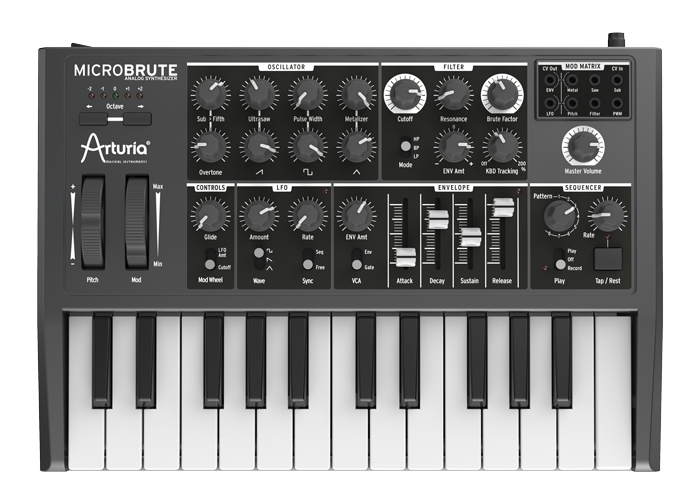
\includegraphics[width=2.5in]{analogSynth}
		\caption{Arturia Microbrute analog synthesizer with digital controls~\cite{analogSynth}. }
		\label{fig:analogSynth}
	\end{figure}
	
	Hybrid synths demonstrate the success of the digital-control-over-analog-audio-circuitry approach. They are readily integrated into computer-based recording studios. The G9 processor takes this hybrid approach to sound generation and applies it to sound processing.
	
	
	
	\section{Project Scope}
	
	Because most recording engineers use equalization (EQ), amplitude dynamic range compression (compressor), and ambiance (reverb), the G9 will have each of those modules. Figure \ref{fig:blockDiagram} shows a block diagram of the G9.
	
	\begin{figure}
		\centering
		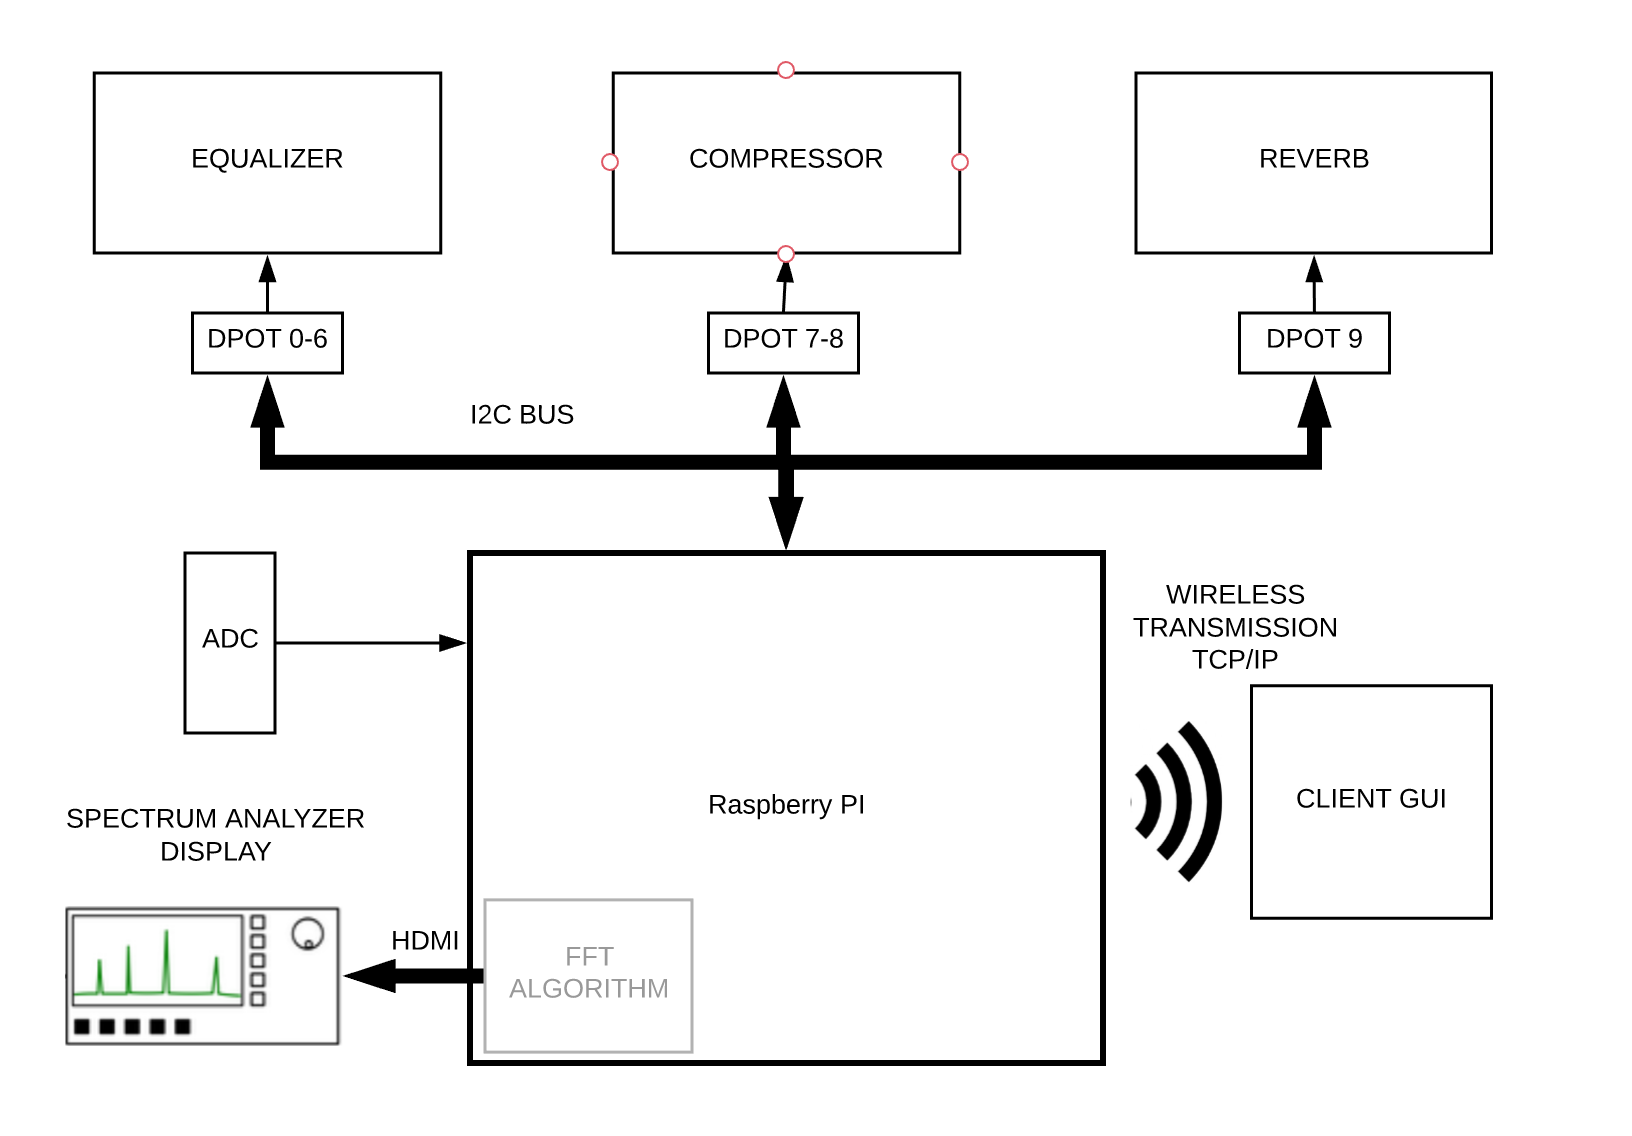
\includegraphics[width=3in]{blockDiagram}
		\caption{Block diagram of the G9. }
		\label{fig:blockDiagram}
	\end{figure}
	
	\subsection{EQ}
	The equalizer in the G9 processor will be based on the Parametric Equalizer and Subwoofer as described by Rod Elliott~\cite{espEq}.  Its circuit diagram is shown in figure \ref{fig:eq}.  This parametric equalizer has four bands that can be cut or boosted up to about 14dB using the 10k potentiometers.  Each of the three 1M potentiometers can be used to select the target frequency for the band.  The Bass can select from 35Hz to 150Hz, the low mid can select 120Hz to 550 Hz, the high mid can select 550 Hz to 2.2kHz, while the treble will be locked on kHz  The op amps that will be used in the circuit are the NE5532, for the input and output op amps, and the TL072 for the others.  The NE5532 produces low noise and so will be needed on the input and output, where the audio signal will be traveling.
	
	The greatest difference between our circuit and the one shown in figure \ref{fig:eq} will be the digital potentiometer ICs in place of the potentiometers.  The ICs will allow for the Raspberry Pi (Rpi) to control the cut and boost as well as the target frequency for the circuit.  Other than that, the power rails will contain additional capacitors to ensure there is little fluctuation in the supply.
	
	
	
	\begin{figure}
		\centering
		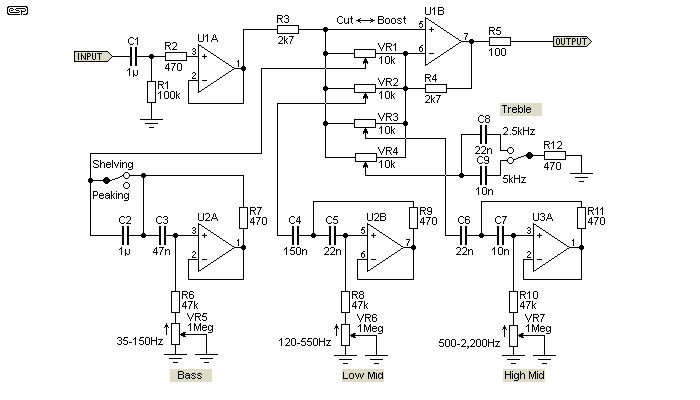
\includegraphics[width=3in]{eq}
		\caption{EQ filter circuit~\cite{espEq}. }
		\label{fig:eq}
	\end{figure}
	
	\subsection{Compressor}
	The compressor will be based on Teletronix LA-2A vacuum tube leveling amplifier. This circuit has two main elements that give it its characteristic sound. First, a gain element is controlled by a combination of an electroluminescent panel and a photo-resistor. The non-linear response curve of that combination results in a very pleasing sound of the gain reduction.  Second, tubes distort the signal in a musical way when the signal level pushes them out of their linear operating zone. Figure \ref{fig:OpticalAttenuator} shows the operating principle of the compressor.
	
	Drip Electronics has developed an updated version of the LA-2A compressor and sells a PCB of their design as well as a PCB for the power supply of the compressor. We already have these PCBs (figures \ref{fig:opto7pcb} and \ref{fig:opto7powerpcb}) and now need to acquire the parts and assemble the unit.
	
	\begin{figure}
		\centering
		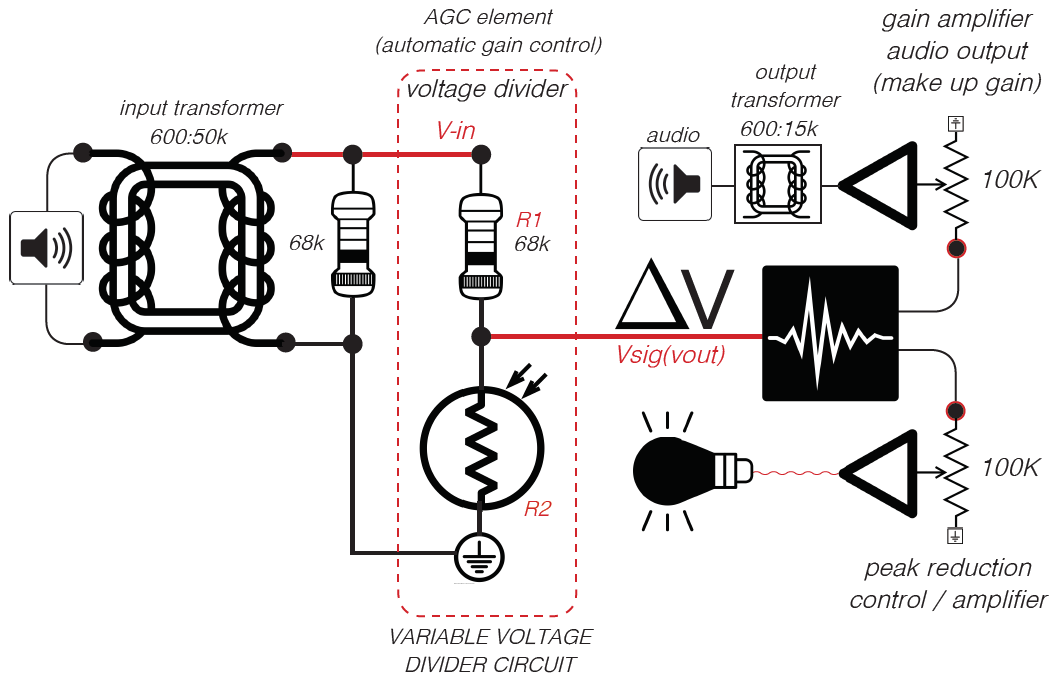
\includegraphics[width=3in]{OpticalAttenuator}
		\caption{Operating principle of the compressor's optical attenuator~\cite{opto7}. }
		\label{fig:OpticalAttenuator}
	\end{figure}
	
	
	\begin{figure}
		\centering
		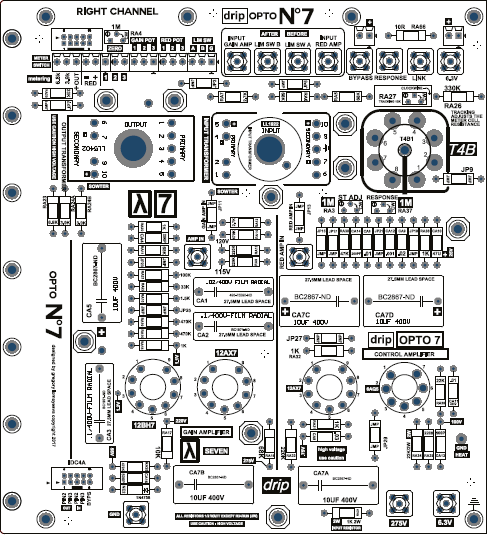
\includegraphics[width=3in]{opto7pcb}
		\caption{PCB of the compressor circuit~\cite{opto7}. }
		\label{fig:opto7pcb}
	\end{figure}

	\begin{figure}
		\centering
		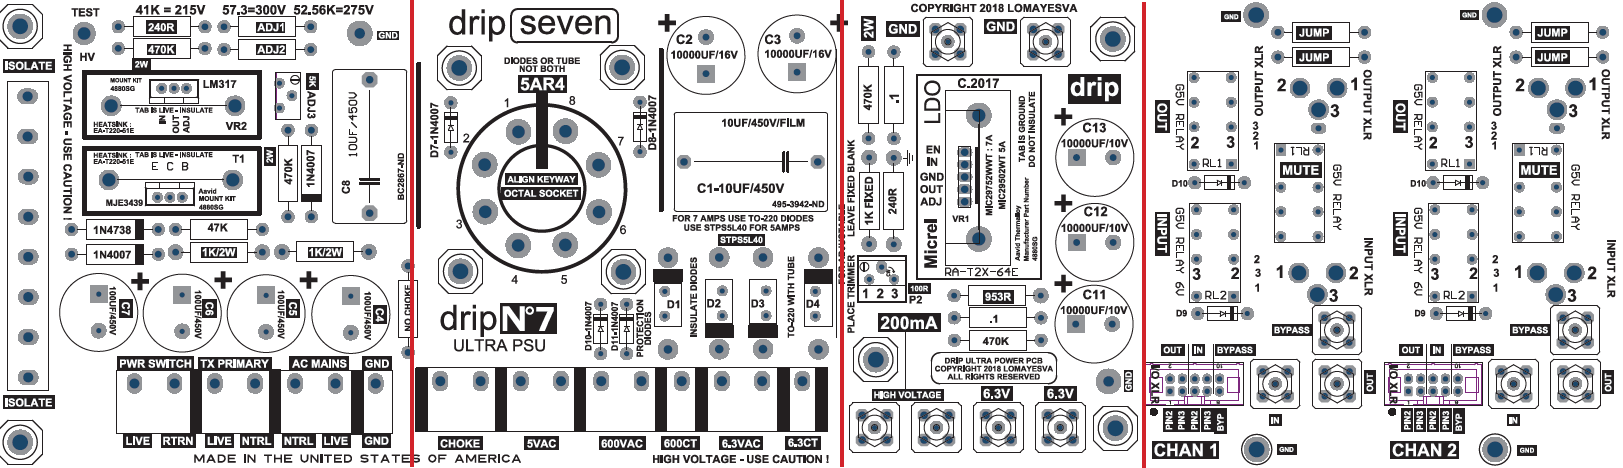
\includegraphics[width=3.4in]{opto7powerpcb}
		\caption{PCB of the compressor's power supply~\cite{opto7}. }
		\label{fig:opto7powerpcb}
	\end{figure}
	

	
	\subsection{Reverb}
	Reverb options are limited in the analog domain. The favored option is to place a loudspeaker in one part of a reverberant chamber and place a microphone in another part. When sound is played through the loudspeaker it is reverberated by the chamber and picked up by the microphone. Reverb of this sort is not feasibly placed inside an enclosure for use in a studio. 
	
	The sound of reverb is generally divided into two parts: early reflections and late reflections~\cite{earlyReflections}. Early reflections are heard as discrete echoes, as when sound bounces off the walls of a chamber. Late reflections are heard after the early reflections as the early reflections build up and fuse into a wash of sound. This part of the reverb is also known as the tail. The time it takes for the tail to fade by 60 dB below the initial sound level is specified as the reverb time. The G9 will combine two methods to achieve a simulation of the chamber's early reflections and reverb tail.
	
	\begin{figure}
		\centering
		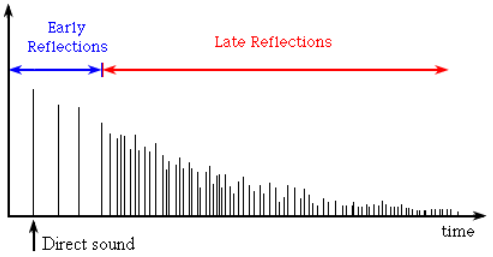
\includegraphics[width=3in]{earlyReflections}
		\caption{Impulse response of a typical reverb signal~\cite{vocalEarlyReflections}. }
		\label{fig:earlyReflections}
	\end{figure}
	
	A hose delay will be used for the early reflections. An amplifier will drive the audio signal through a balanced armature driver, like those used by in-ear monitors. The driver will be coupled to one end of a thin hose or tube. A microphone will be coupled to the other end. Sound played at one end will travel through the hose and be picked up by an electret microphone at the other end. Feedback can be used for sound reflections at a multiple of the delay time; multiple hose rigs can be used for specific reflections.
	
	An amplifier will take the signal from the microphone and drive it through a pair of springs to generate the dense, diffuse reflections that happen in a reverberant chamber after the sharp early reflections decay into a wash of sound. Figure \ref{fig:reverbBlock} shows a diagram of the reverb section of the G9. Amplifier schematics for the reverb are shown in figure \ref{fig:espMicPreSpringDrive}.
	
	\begin{figure}
		\centering
		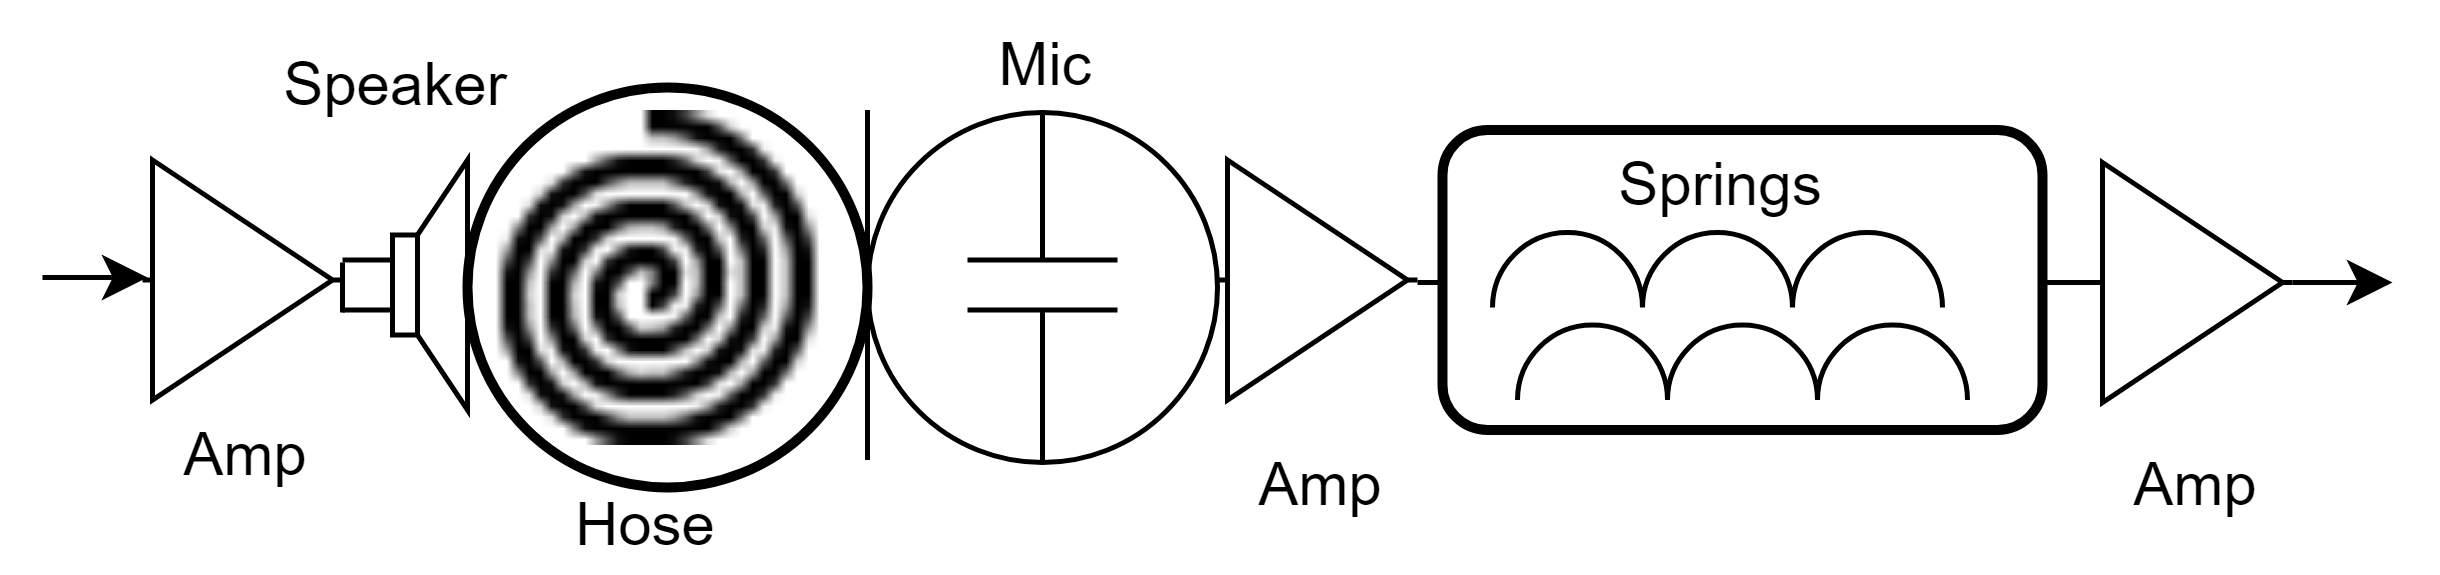
\includegraphics[width=3in]{reverbBlock}
		\caption{Diagram of the reverb section }
		\label{fig:reverbBlock}
	\end{figure}
	
	
	
	\begin{figure}
		\centering
		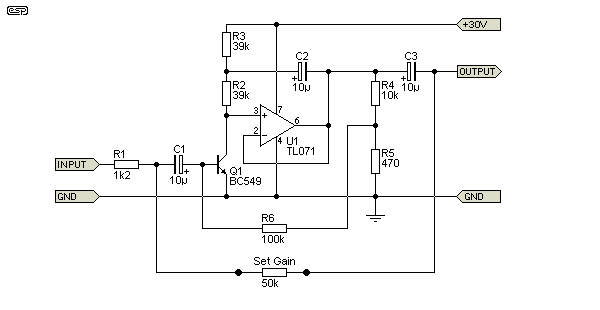
\includegraphics[width=3in]{espMicPreSpringDrive}
		\caption{Reverb amplifiers~\cite{espMicPreSpringDrive}. }
		\label{fig:espMicPreSpringDrive}
	\end{figure}

	\subsection{Enclosure}
	The G9 processor will be contained in an enclosure made of both metal and a clear acrylic.  The compressor circuit requires a metal casing to connect to ground.  This allows for greater safety with the high voltages introduced in that circuit for the tube amps.  The compressor and the rest of the project will be contained in a case made out of laser cut acrylic.  The clear polished look will make the internal circuits visible, and give a nice clean look for the enclosure itself.  The only components that will be outward facing are the power supply cord, the audio jacks, the LEDs to display the current signal level, and the small HDMI screen we are using to display the frequency spectrum of the audio signal.  
	
	The G9 processor will plug into a standard wall plug to generate the voltages it needs using a few different power supplies.  We need to ensure we have the low voltage +30V, +/- 15V,  and +/- 5V for the Rpi and filters, and the high voltage for the compressor's tube circuit.  The HDMI screen is a 5'' screen that we will be connecting to the Rpi to display the frequency spectrum of the audio signal as it runs through the processor.  
	
	
	
	\subsection{Digital Control}
	Digital control over each module will be dictated by the user through a Graphical User Interface which communicates with the Rpi over a TCP network.  The Rpi will operate a server which may grant a client request or update the client on changes to physical controls of the G9 enclosure.  The client represents the user and the changes made by the user to the user interface will become requests to the server.  In addition to simply granting requests, the Rpi will schedule processes such as I2C communication tasks, spectrum analysis tasks and client request tasks in a manner that prioritizes responsiveness to the user.  Additionally, the physical controls of the G9 (dials) will represent the current setting of the input and output levels with an array of LEDs surrounding each control.  Requested changes that are granted to the client will be reflected in the LEDs to keep software and hardware interfaces in sync.  Because each module has different parameters, the physical interface and software interface can dynamically change to represent the settings of each respective module.
	
	
	
	\begin{figure}
		\centering
		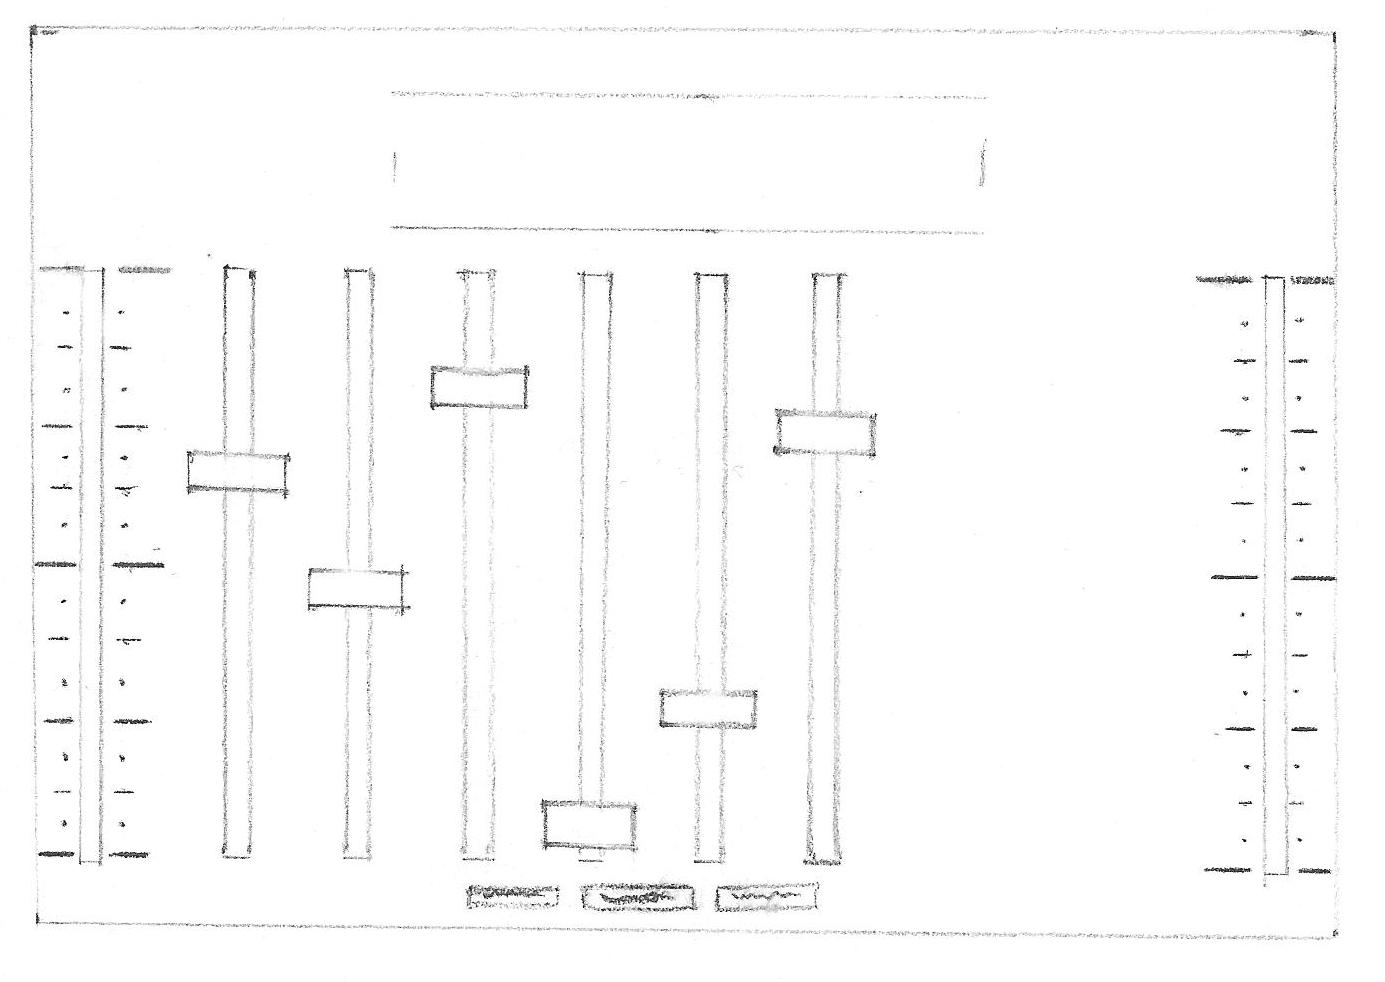
\includegraphics[width=2.5in]{gui}
		\caption{Mockup of the G9's GUI. }
		\label{fig:gui}
	\end{figure}
	
	
	\section{Digital Potentiometers}
	To maintain an analog signal path while simultaneously modifying analog parameters with digital controls, each audio filter will be using digital potentiometer ICs.  Digital potentiometers can produce very similar result to analog potentiometers, however they also allow for digital control over a serial interface, I2C in our case.  The G9 processor will be using the AD5144 and the AD5342 digital potentiometers.  The first has 4 potentiometers on board, allowing us to use fewer I2C lines, and the second only has 2.  We need to use the second as well because the 1M digital potentiometers do not come in packages of more than 2. These digital potentiometers allow for us to alter the parameters of the analog filters, in the case of the EQ, we can select the target frequencies and the cut or boost for those frequencies.
	

	Figure \ref{fig:g9Enclosure} shows a mockup of the G9's enclosure. It will have LED meters showing input and output signal levels, an LED meter showing the compressor's gain reduction, and an LED meter showing the reverb's wet/dry signal balance. It will also have two rotary encoders to adjust the signal level going into the processor and the signal level coming out of the processor. The rotary encoders will allow for the changes to be saved with the GUI as well as for the state to be loaded easily.
	\begin{figure}
		\centering
		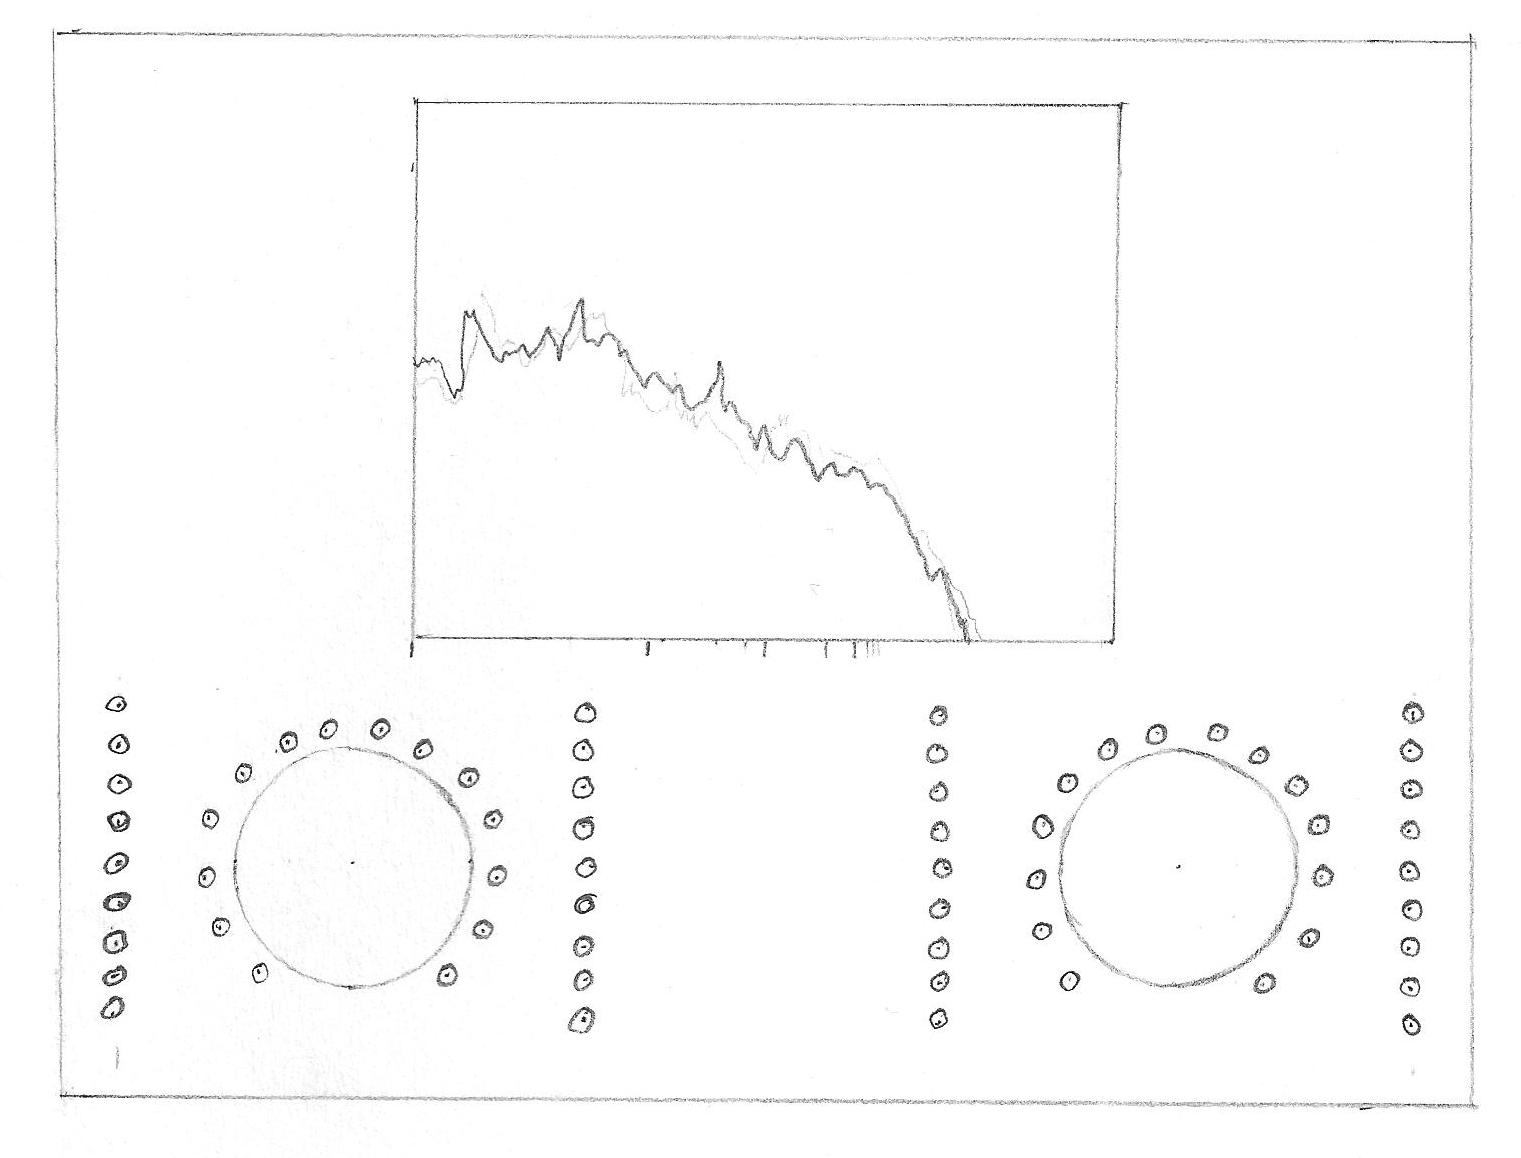
\includegraphics[width=2.5in]{g9Enclosure}
		\caption{Mockup of the G9's enclosure. }
		\label{fig:g9Enclosure}
	\end{figure}
	
	
	\begin{figure}
		\centering
		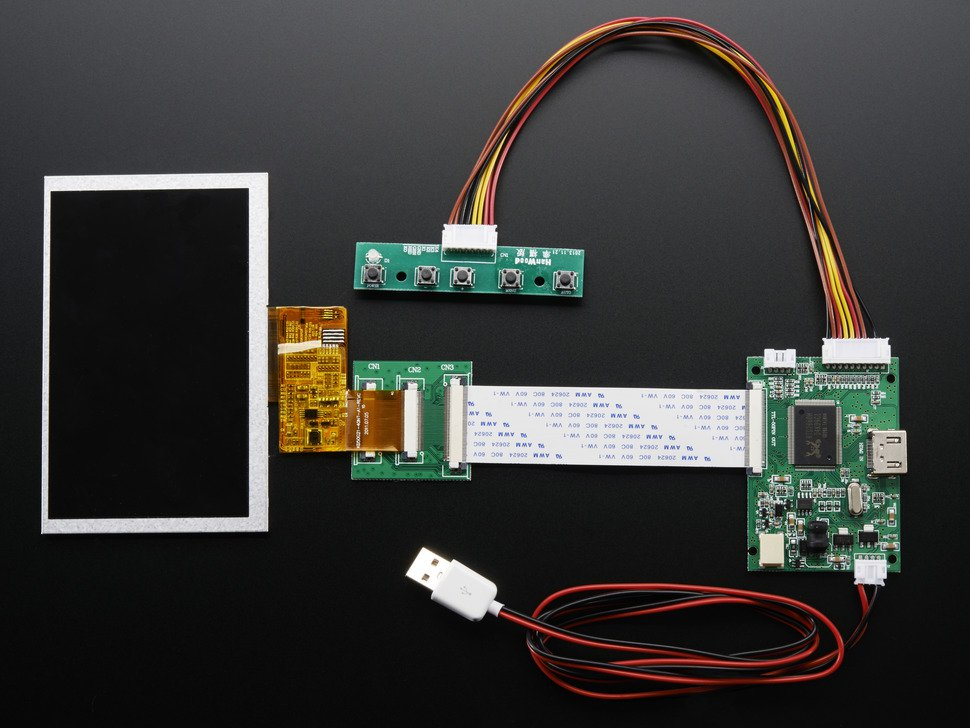
\includegraphics[width=3in]{hdmiDisplay}
		\caption{HDMI display for the enclosure \cite{hdmiDisplay}. }
		\label{fig:hdmiDisplay}
	\end{figure}

	    
	\section{Design Challenges and Risks}
	In designing the G9 Processor, we have found several aspects of the project that may prove to be a challenge.  What follows is a list of these challenges and an explanation of each:
	\begin{itemize}
		\item \textbf{Latency}: With the Rpi performing as many tasks as it will be, I2C, network communication, audio signal analysis, the latency between changing a parameter on the GUI and the change propagating to the device may be noticeable.
		\item \textbf{Frequency Spectrum Display}: Although we have found a C library that can perform the necessary FFT on the incoming audio signal, we still need to find a way to place the result into a nice format such that it can be display on the small HDMI screen we have.
		\item \textbf{I2C Communication}: I2C is a simple communication protocol, but we will be filling the I2C lines on our Rpi and it may be a small challenge to ensure we address each device and the registers in each device correctly.
		\item \textbf{Multiple Power Rails}: We are using several different circuits and many of the components we are using require different power supplies.  Coordinating each of the different power rails may prove to be a challenge.
		\item \textbf{High Voltages}: The G9 processor's compressor circuit is built using tube amps.  They require very high voltages to function, on the ranges of 600 VAC and 250 VDC.  Ensuring these voltages will not cause problems, and that we stay safe when using them will be a challenge.
	\end{itemize}
	
	There are a number of risks with the G9 processor, and the first is deals with the compressor circuit.  When building the compressor we will need to ensure care is taken so that none of the team members are injured and that the circuit survives.  The primary caution will be to keep it unconnected to the power until the circuit is fully constructed and has been tested for shorts.  In the event that the circuit is burnt out by the high voltages we can resort to using a solid state compressor in the processor.  Ordering parts and soldering provide another risk.  The parts must be ordered early and with spares to account for long delivery times and burning out components as we construct the processor.  The last risk is that the Raspberry Pi Zero W may not be able to perform all the tasks we need it to accomplish.  It may not have enough power to perform the FFT or may not be able to handle the I2C communication.  In this case, we can add one of our STM32F0 discovery boards to the project to ensure it will be completed on time.
	
	\section{Milestones and Progress}
	The G9 processor is to be completed by the end of November of 2018.  On the path towards that completion, we need to assemble and test each of the filters and then interface with the contained digital potentiometers with the Rpi.  Additionally, a GUI will need to be designed and communicating with the Rpi and the Rpi needs to perform an FFT on the audio signal to display the frequency spectrum.  
	
	The first of these steps, constructing each of the filters and then getting some communication with the Rpi is planned to completed over the summer.  At the start of the fall semester, we plan on having individual parts all constructed.  We will spend the semester bringing everything together and debugging the code we have.
	
	We have made a little progress in achieving this goal.  The EQ circuit has been built and tested and its next step is constructing a PCB.  The compressor's PCBs have already been acquired and the transformers are on their way.  Its other parts still need to be ordered.  The reverb circuit has been designed, though we only have the hose and the spring for it.  The Raspberry Pi Zero W has been ordered and is on its way, and we have found a C library that we can use to perform the FFT to display on a small HDMI screen we already have.
	
	\subsection{Tasks}
	
	Tables \ref{tab:owners} and \ref{tab:milestones} give a broad overview of responsibilities in the project. Everyone will be flexible regarding the work they do and frequent communication is vital, but final decisions regarding components will fall to the component owner.
	
	\begin{table}[H]
		\centering
		\caption{Component Owners}
		\label{tab:owners}
		\begin{tabular}{l|l}
			Component                     & Owner \\ \hline
			EQ                     & Jeremy \\
			Compressor             & Steve  \\
			Reverb                 & Steve  \\
			GUI                    & Nick   \\
			Spectrum display       & Nick   \\
			Enclosure and controls & Jeremy
		\end{tabular}
	\end{table}

	\begin{table}[H]
		\centering
		\caption{Milestones}
		\label{tab:milestones}
		\begin{tabular}{l|l}
			Month     & Milestone                       \\ \hline
			June      & Simple GUI, EQ                  \\
			July      & Reverb, I2C with digipots       \\
			August    & Compressor                      \\
			September & Enclosure and Hardware complete \\
			October   & Software fully functional       \\
			November  & Debugging                      
		\end{tabular}
	\end{table}
	


	
	\section{Testing Plan}
	The G9 is highly modular. Each piece can be tested on its own to ensure it functions correctly before attempting to combine all the elements together. GUI, CPU, FPGA, display, EQ, compressor, reverb will all be tested on their own. When each component is functioning correctly on its own, then the pieces will be connected together one-by-one and tested.
	
	\section{Demo}
	A base demo of the G9 will consist of a sound playback device being plugged into the G9, and the output of the G9 will be plugged into a sound system. A separate room for the demo is desired since it might get loud. Each of the three sound processors will be demonstrated in turn by adjusting their parameters one by one on the GUI and listening to how the sound changes on the playback system. A more detailed demo will consist of an in-depth presentation of how the GUI, control system, analog processors, and information display all work together.
	
	\section{Mentors and Resources}
	Through this initial design phase, Dr. Erik Brunvand, Dr. Pierre-Emmanuel Gaillardon, and Dr. Angela Rassmussen have provided valuable advice. We anticipate needing more guidance from them during the construction phase. Adam Weinstein provided excellent critiques of our writing and we'll be sad to lose him as the TA, if in fact that is the case moving forward to fall semester. Drip Electronics provides support for assembling the compressor. There are many online forums that cover various aspects of our project and we will be utilizing them.
	
	
	
	\section{Summary}
	Analog audio processors provide minimal delay, however they do not allow for digital control.  Digital processors provide digital control, but they can introduce an audible delay into the audio signal.  The G9 audio processor will combine minimal delay of an analog signal path with the digital control of a computer to provide ease of use.  Some of the main benefits include: restorable sound settings, integration with other digital sound equipment, and wireless control of sound settings.
	
	The G9 processor consists of three audio filters. The first is a simple parametric equalizer that allows for 4 band selection.  We will be using the equalizer circuit as given by Elliott Sound Products~\cite{espEq}.  The second, a compressor circuit, uses tube amps and requires high voltages to utilize the amp.  We will be using the circuit from Drip Electronics~\cite{opto7}. The last filter is the reverb circuit  To create this circuit, we plan on using a hose to give a small delay to produce early reverb reflections, and then a spring to produce late reverb reflections.
	
	A Raspberry Pi W microprocessor will integrate each of the audio filters, a control server, and a frequency spectrum analyzer.  Hosting a server, the Rpi will control each of the audio filters as requested by a wireless GUI connected to it.  The filters can be controlled by using I2C communications with digital potentiometer ICs that are contained within.  C code that can run the necessary spectrum analysis, contained in the FFTW C library, will be running on the Rpi and providing its data to an HDMI driven display on the enclosure of the G9.  The spectrum analyzer will display the frequency spectrum to a 256-point resolution. We plan on completing the processor's individual components over the summer and bringing everything together as fall semester begins. 
	
	
	
	\appendix
	Tables \ref{tab:compressorParts} - \ref{tab:powerSupplies} list additional parts needed for the project. It is anticipated that more parts will be required as needed, but the ones listed include the vast majority of them. The main vendors for the parts will include Tube Depot, DigiKey, Mouser, and Arrow.
	
	
	
	\begin{table}[]
		\centering
		\caption{Compressor Parts}
		\label{tab:compressorParts}
		\begin{tabular}{l|l}
			Part                           & Qty. \\\hline
			Schottky Diode 1200V, 5A              & 2          \\
			450V 40uF                             & 4          \\
			50volts 47uF                          & 1          \\
			500pF 500V                            & 2          \\
			150pF 500V                            & 2          \\
			2watts 1Mohms                         & 2          \\
			Lamp 65VAC .7mA NE-2E                 & 1          \\
			XLR Connectors 3Pin male                & 1          \\
			XLR Connectors 3Pin female              & 1          \\
			AC Power Socket and fuse              & 1          \\
			Terminals LUG LOCK                    & 10         \\
			AC Power Cord 18AWG                   & 1          \\
			3/8"SQ 1Mohms Multi Turn              & 3          \\
			1/2watt 220K                          & 5          \\
			1/2watt 33K                           & 3          \\
			1/2watt 330K                          & 1          \\
			1/2watt 3.9K                          & 2          \\
			1/2watt 2.7K                          & 1          \\
			3watts 4.7Kohms                       & 1          \\
			3 WATT 22K                            & 1          \\
			1watt 24K                             & 1          \\
			Fuse 250V 1A Slo-Blo                  & 4          \\
			450V 10uF                             & 1          \\
			3/8"SQ 100Kohms Multi Turn            & 1          \\
			Rectifier Vr/1000V Io/1A              & 2          \\
			400V .1uF                             & 2          \\
			400Volts 100000pF                     & 4          \\
			400Volts 22000pF                      & 3          \\
			600Volts 1000pF                       & 1          \\
			400Volts 10000pF                      & 3          \\
			Terminal Blocks 10P 5.08mm 90DEG      & 1          \\
			Terminal Blocks 3P 5.08mm 90DEG       & 3          \\
			Terminal Blocks 2P 5.08mm 90DEG       & 3          \\
			3watts 470K                           & 1          \\
			Terminal Blocks 2P 5.08mm 40DEG       & 5          \\
			1/2watt 47K                           & 1          \\
			1/2watt 10K                           & 2          \\
			1/2W 68K                              & 4          \\
			1/2watt 100K                          & 1          \\
			1/2watt 470K                          & 5          \\
			2watts 100ohms                        & 2          \\
			Rotary Switches                       & 1          \\
			2watts 3.9K                           & 1          \\
			2watts 6.8K                           & 1          \\
			1watt 22K                             & 2          \\
			1watt 1.5K                            & 1          \\
			Audio output transformer              & 1          \\
			Audio input transformer               & 1          \\
			Power transformer                     & 1          \\
			Photo cell                            & 1          \\
			Rectifier tube                        & 1          \\
			Amplifier tube                        & 1          \\
			Amplifier tube                        & 2          \\
			Amplifier tube                        & 1          \\
			8 pin tube socket for 5AR4 and T4B    & 2          \\
			9 pin tube socket for 12BH7 and 12AX7 & 3          \\
			7 pin tube socket for 6AQ5            & 1         
		\end{tabular}
	\end{table}
	
	\begin{table}[]
		\centering
		\caption{Reverb Parts}
		\label{tab:reverbParts}
		\begin{tabular}{ll|l}
			Part                             &  & Qty. \\ \hline
			
			1/2watt 1k2                               &  & 3          \\
			1/2watt 39k                               &  & 6          \\
			1/2watt 10k                               &  & 3          \\
			1/2watt 470                               &  & 3          \\
			1/2watt 100k                              &  & 3          \\
			100k potentiometer                &  & 3          \\
			25V 10u                               &  & 9          \\
			BC549 transistor                  &  & 3          \\
			TL071 op-amp                      &  & 3          \\
			Etymotic ER4 drivers              &  & 1          \\
			Panasonic electret mic            &  & 1          \\
			100' Orbit drip irrigation tubing &  & 1          \\
			Accutronics spring reverb tank    &  & 1         
		\end{tabular}
	\end{table}


	\begin{table}[]
		\centering
		\caption{EQ Parts}
		\label{tab:eq}
		\begin{tabular}{l|l}
			Part                               & Qty. \\ \hline
			1/2watt 100k  & 1 \\ 
			1/2watt 470   & 5 \\
			1/2watt 2k7   & 2 \\
			1/2watt 100   & 1 \\
			1/2watt 47k   & 3 \\
			1u            & 2 \\
			22n           & 3 \\
			10n           & 2 \\
			47n           & 1 \\
			150n          & 1 \\
			NE5532 op-amp & 2 \\
			TL072 op-amp  & 3
		\end{tabular}
	\end{table}

	\begin{table}[]
		\centering
		\caption{Enclosure Parts}
		\label{tab:enclosure}
		\begin{tabular}{l|l}
			Part                               & Qty. \\ \hline
			HDMI 5" 800x480    & 1  \\
			Raspberry Pi Zero W    & 1  \\
			Rotary Encoder     & 1  \\
			MAX7219 LED driver & 1  \\
			Red LED            & 4  \\
			Yellow LED         & 6  \\
			Green LED          & 11 \\
			1/2watt 470        & 6  \\
			3 rack space enclosure & 2
		\end{tabular}
	\end{table}


	\begin{table}[]
		\centering
		\caption{Power Supplies}
		\label{tab:powerSupplies}
		\begin{tabular}{l|l|l}

			Model     & Manufacturer     & Notes          \\\hline
			CUT75-5FF & TDK Lambda       & +/- 15V, +5V    \\
			ZPSA40-30 & TDK Lambda       & +30V           \\
			Ultimate  & Drip Electronics & 6.3VAC, 550VAC \\
			Fifth Rail  & Group 9 & -5V
		\end{tabular}
	\end{table}


	

	
	% Can use something like this to put references on a page
	% by themselves when using endfloat and the captionsoff option.
	\ifCLASSOPTIONcaptionsoff
	\newpage
	\fi
	
	
	
	\bibliographystyle{ieeetran}
	\bibliography{g9}
\end{document}
